\chapter*{Part B\@: Autoencoders}

\section*{Introduction}

This part of the assignment aims to implement an autoencoder on the full MNIST
dataset.

\section*{Stacked Denoising Autoencoder}

The stacked denoising autoencoder consists of three hidden layers with 900, 625
and 400 neurons respectively. The following plot shows the training cost of the
autoencoder.

\begin{center}
    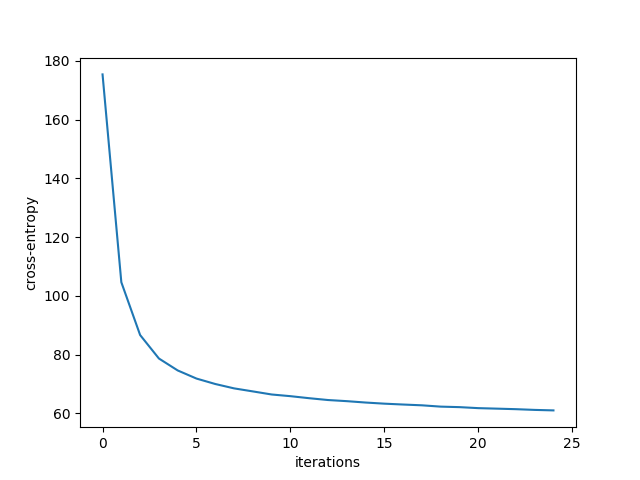
\includegraphics[width=\imgw]{project_2b_train}
\end{center}

The following images show 100 samples of weights learned at each layer.

\begin{longtabu}{X[c]X[c]}
    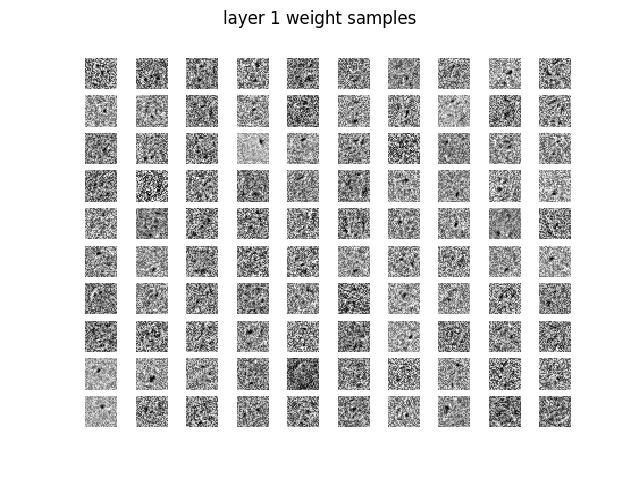
\includegraphics[width=\imgwt]{project_2b_weight1} &
    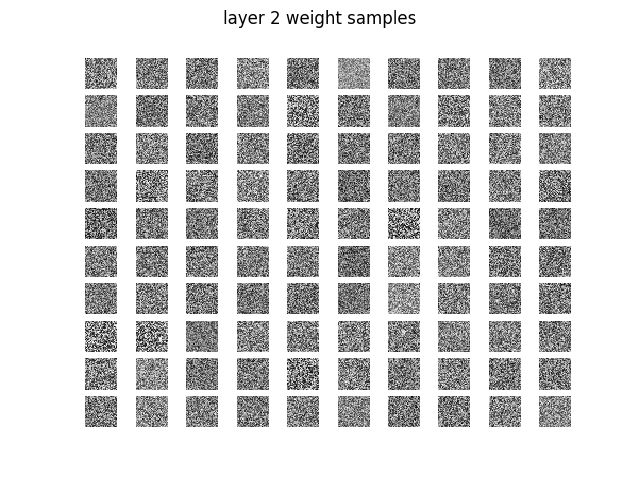
\includegraphics[width=\imgwt]{project_2b_weight2} \\
    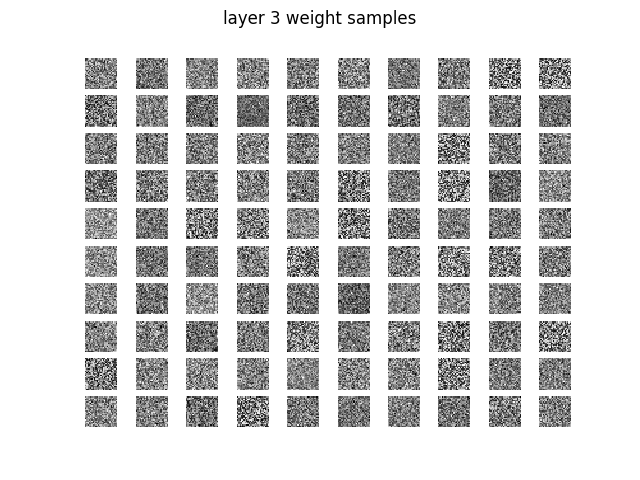
\includegraphics[width=\imgwt]{project_2b_weight3}
\end{longtabu}

100 test images are chosen at random; the images and their reconstructions are
shown below.

\begin{longtabu}{X[c]X[c]}
    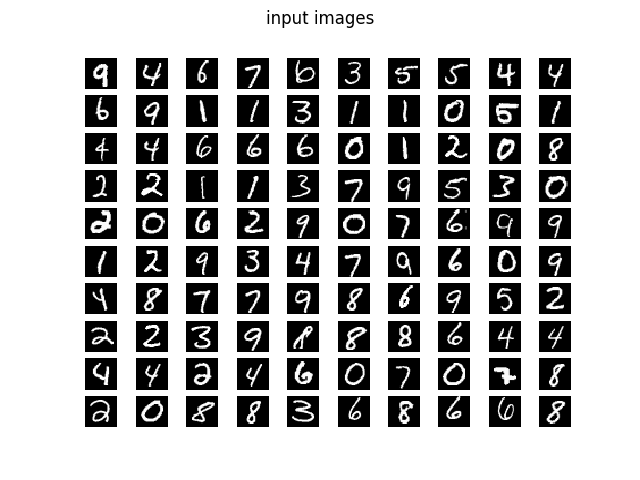
\includegraphics[width=\imgwt]{project_2b_input} &
    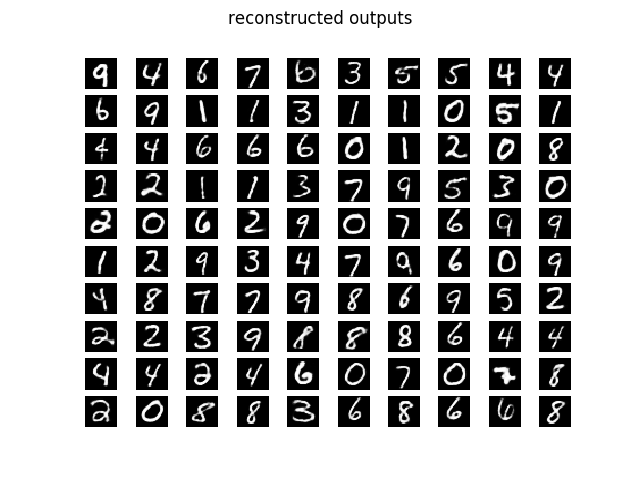
\includegraphics[width=\imgwt]{project_2b_output}
\end{longtabu}

The hidden layer activations are shown below.

\begin{longtabu}{X[c]X[c]}
    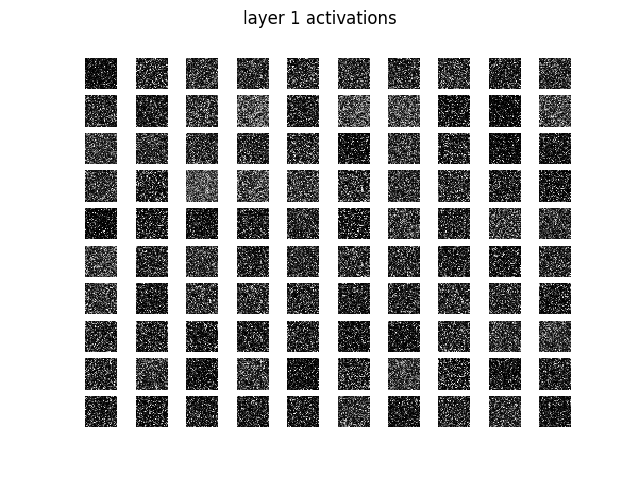
\includegraphics[width=\imgwt]{project_2b_layer1} &
    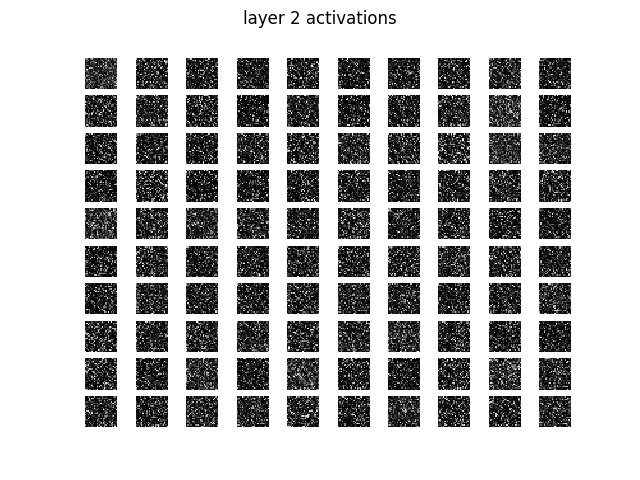
\includegraphics[width=\imgwt]{project_2b_layer2} \\
    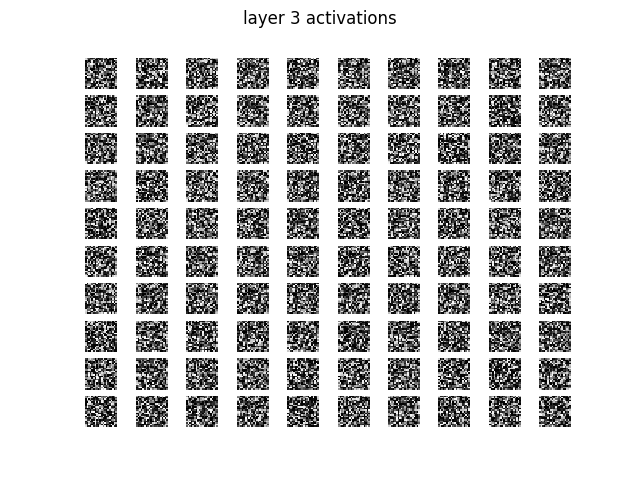
\includegraphics[width=\imgwt]{project_2b_layer3}
\end{longtabu}

\section*{Feedforward Neural Network on Autoencoder}

We added a softmax and an output layer to the stacked denoising autoencoder
described above, to make a classifier on MNIST data. The training cost is shown 
below.

\begin{center}
    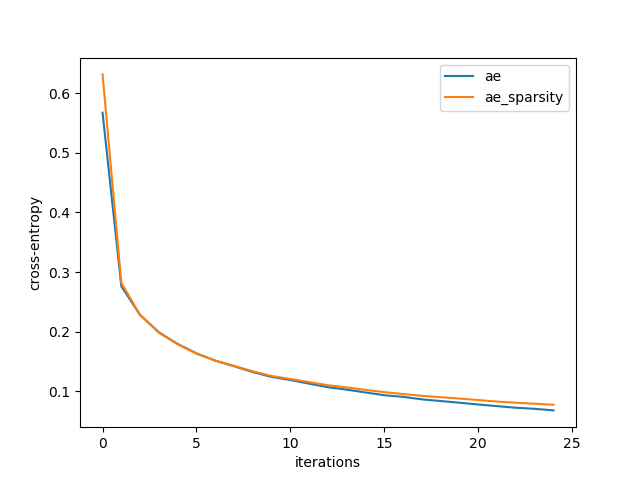
\includegraphics[width=\imgw]{project_2b_train_ffn}
\end{center}

The test accuracy is shown below; the classifier achieves 97.2\% accuracy after
25 epochs.

\begin{center}
    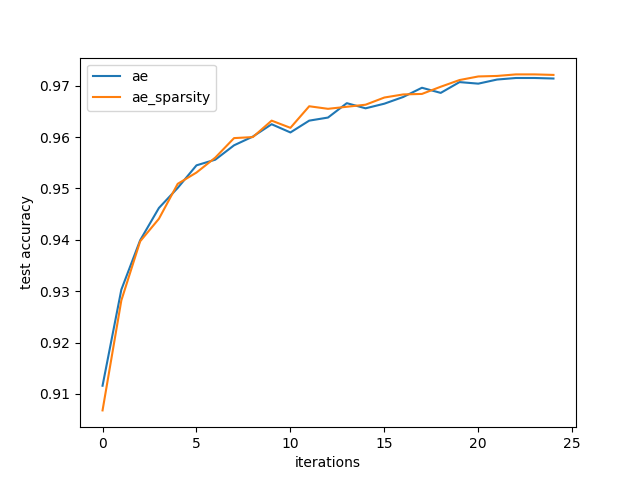
\includegraphics[width=\imgw]{project_2b_test_ffn}
\end{center}